\chapter{Neural Networks}
In this chapter, we discuss \href{https://en.wikipedia.org/wiki/Artificial_neural_network}{neural networks}.
Many of the most visible breakthroughs in artificial intelligence have been achieved through the use of neural
networks: 
\begin{enumerate}
\item The current system used by Google to \href{https://translate.google.com}{automatically translate} web
      pages is called 
      ``\href{https://en.wikipedia.org/wiki/Google_Neural_Machine_Translation}{Google Neural Machine
        Translation}''
      and,  as the name suggests, is based on neural networks.
\item \href{https://www.deepl.com/translator}{DeepL} is another translator that is based on deep neural networks.      
\item \href{https://de.wikipedia.org/wiki/AlphaGo}{AlphaGo} uses neural networks together with tree search
      \cite{silver:2016}.  It has \href{https://en.wikipedia.org/wiki/AlphaGo_versus_Ke_Jie}{beaten} 
      beaten the world champion \href{https://en.wikipedia.org/wiki/Ke_Jie}{Ke Jie} in the game of
      \href{https://en.wikipedia.org/wiki/Go_(game)}{Go}.
\item \href{https://www.tensorflow.org/tutorials/image_recognition}{Image recognition} is best done via neural networks.
\item \href{https://en.wikipedia.org/wiki/Autonomous_car}{Autonomous driving} makes heavy use of neural networks.
\end{enumerate}
The list given above is far from being complete.  In this chapter, we will only discuss \blue{feedforward} 
neural networks.  Although recently 
\href{https://en.wikipedia.org/wiki/Recurrent_neural_network}{recurrent neural networks} have gotten a lot of
attention, these type of neural networks are more difficult to train and are therefore beyond the scope of this
introduction.  The rest of this chapter is strongly influenced by the online book 
\\[0.2cm]
\hspace*{1.3cm}
\href{http://neuralnetworksanddeeplearning.com/index.html}{http://neuralnetworksanddeeplearning.com/index.html}
\\[0.2cm]
that has been written by Michael Nielsen \cite{nielsen:2015}.  This book is easy to read, carefully written, and
free to access.  I recommend this book to anybody who wants to dive deeper into the fascinating topic of neural
networks.

\section{Feedforward Neural Networks}
A neural network is built from \blue{neurons}.  Neural networks are inspired by biological 
\href{https://en.wikipedia.org/wiki/Neuron}{neurons}.  However, in order to understand artificial neural
networks it is not necessary to know how biological neurons work and it is definitely not necessary to
understand how networks of biological neurons, i.e.~brains, work\footnote{
  Actually, when it comes to brains, although there are many speculations, surprisingly little is known for a fact.  
}.  
Instead, we develop a mathematical
abstraction of neurons that will serve as the foundation of the theory developed in this chapter.
At the abstraction level that we are looking at neural networks, a single neuron with $n$ inputs is defined as
a pair $\langle \mathbf{w}, b\rangle$ where the 
vector $\mathbf{w} \in \mathbb{R}^m$ is called the \blue{weight vector} and the number $b \in \mathbb{R}$ is called the \blue{bias}.  
Conceptually, a neuron is a function $p$ that maps an input vector $\mathbf{x} \in \mathbb{R}^m$ into the
interval $[0,1]$.  This function is defined as follows:
\\[0.2cm]
\hspace*{1.3cm}
$\ds p(\mathbf{x}; \mathbf{w}, b) := a(\mathbf{x} \cdot \mathbf{w} + b)$,
\\[0.2cm]
where $a$ is called the \blue{activation function}.  In our applications, we will always use the sigmoid
function as our activation function, i.e.~we have
\\[0.2cm]
\hspace*{1.3cm}
$\ds a(t) := S(t) = \frac{1}{1 + \exp(-t)}$.
\\[0.2cm]
The function $p$ modelling the neuron can be written more explicitly using index notation.  If
\\[0.2cm]
\hspace*{1.3cm}
$\mathbf{w} = \langle w_1, \cdots, w_m \rangle^\top$ 
\\[0.2cm]
is the weight vector and 
\\[0.2cm]
\hspace*{1.3cm}
$\mathbf{x} = \langle x_1, \cdots, x_m \rangle^\top$
\\[0.2cm]
is the input vector, then we have
\\[0.2cm]
\hspace*{1.3cm}
$\ds p(\mathbf{x}; \mathbf{w}, b) = S\left(\biggl(\sum\limits_{i=1}^m x_i \cdot w_i\biggr) + b\right)$.
\\[0.2cm]
If we compare $p(\mathbf{x}; \mathbf{w}, b)$ 
to a similar function appearing in the last chapter, you will notice 
that so far a neuron works just like logistic regression.  The only difference is that the bias $b$
is now explicit in our notation.  In logistic regression, we had assumed that the first component $x_1$ of our
feature vector $\mathbf{x}$ was always equal to $1$.  This assumption enabled us to incorporate the bias $b$ into the
weight vector $\mathbf{w}$.

A \blue{feedforward neural network} is a layered network of neurons.  Formally, the \blue{topology} of a neural network is
given by a number $L \in \mathbb{N}$ and a list $[m(1), \cdots, m(L)]$ of $L$ natural numbers.  The number
$L$ is called the \blue{number of layers} and for $i \in \{2,\cdots,L\}$ the number $m(i)$ is the number of
neurons in the $l$-th layer.  The first layer is called the \blue{input layer}.  The input layer does not contain
neurons but instead just contains \blue{input nodes}.  The last layer (i.e.~the
layer with index $L$) is called the \blue{output layer} and the remaining layers are called 
\blue{hidden layers}.  If there is more than one hidden layer, the neural network is called a
\blue{deep neural network}.  Figure \ref{fig:neural-network.png} on page \pageref{fig:neural-network.png} shows
a small neural network with two hidden layers.

\begin{figure}[!h]
  \centering
   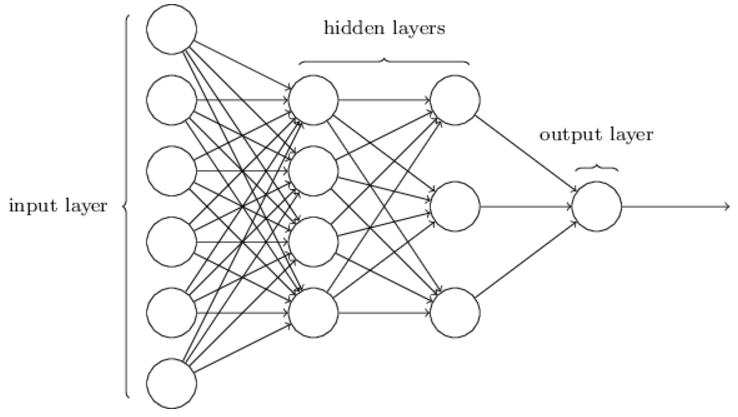
\epsfig{file=Figures/neural-network.png,scale=0.8}
   \caption{A neural network taken from the book by
     \href{http://neuralnetworksanddeeplearning.com}{Michael Nielsen}\cite{nielsen:2015}.}
  \label{fig:neural-network.png}
\end{figure}


As the first layer is the input layer, the \blue{input dimension} is defined as
$m(1)$.  Similarly, the \blue{output dimension} is defined as $m(L)$.
Every node in the $l$-th layer is connected to every node in the $(l+1)$-th layer via a \blue{weight}.
The weight $w_{j,k}^{(l)}$ is the weight of the connection from the $k$-th neuron in layer $l-1$ to
the $j$-th neuron in layer $l$.  The weights in layer $l$ are combined into the \blue{weight matrix} $W^{(l)}$ of
the layer $l$: This matrix is defined as
\\[0.2cm]
\hspace*{1.3cm}
$\ds W^{(l)} := \bigl( w_{j,k}^{(l)} \bigr)$.
\\[0.2cm]
Note that $W^{(l)}$ is an $m(l) \times m(l-1)$ matrix, i.e.~we have
\\[0.2cm]
\hspace*{1.3cm}
$\ds W^{(l)} \in \mathbb{R}^{m(l) \times m(l-1)}$.
\\[0.2cm]
The $j$-th neuron in layer $l$ has the \blue{bias} $b_j^{(l)}$.  These biases of layer $l$ are combined into
the \blue{bias vector}
\\[0.2cm]
\hspace*{1.3cm}
$\mathbf{b}^{(l)} := \langle b_1^{(l)}, \cdots, b_{m(l)}^{(l)} \rangle^\top$.
\\[0.2cm]
Then, the \blue{activation} of the $j$-th neuron
in layer $l$ is denoted as $a_j^{(l)}$ and is defined recursively as follows:
\begin{enumerate}
\item For the input layer we have
      \begin{equation}
        \label{eq:feedforward1}
       a^{(1)}_j := x_j.
       \tag{FF1}
      \end{equation}
      To put it differently, the input vector $\mathbf{x}$ is the activation of the input nodes.
\item For all other layers we have
      \begin{equation}
         \label{eq:feedforward2}
         a_j^{(l)}(\mathbf{x}) := 
             S\left(\Biggl(\sum\limits_{k=1}^{m(l-1)} w_{j,k}^{(l)}\cdot a_k^{(l-1)}(\mathbf{x})\Biggr) + b_{j}^{(l)}\right) 
        \quad \mbox{for all $l \in \{2, \cdots, L\}$}.
       \tag{FF2}
\end{equation}
\end{enumerate}
The \blue{activation vector} of layer $l$ is defined as
\\[0.2cm]
\hspace*{1.3cm}
$\mathbf{a}^{(l)} := \langle a_1^{(l)}, \cdots, a_{m(l)}^{(l)} \rangle^\top$.
\\[0.2cm]
The output of our neural network for an input $\mathbf{x}$ is given by the neurons in the output
layer,  i.e.~the output vector 
$\mathbf{o}(\mathbf{x}) \in \mathbb{R}^{m(L)}$ is defined as 
\\[0.2cm]
\hspace*{1.3cm}
$\mathbf{o}(\mathbf{x}) := \langle a^{(L)}_1(\mathbf{x}), \cdots, a^{(L)}_{m(L)}(\mathbf{x}) \rangle^\top = \mathbf{a}^{(L)}(\mathbf{x})$.
\\[0.2cm]
Note that the equations (\ref{eq:feedforward1}) and (\ref{eq:feedforward2}) describe how information propagates
through the neural network: 
\begin{enumerate}
\item Initially, the input vector $\mathbf{x}$ is given and stored in the input layer of the neural network:
      \\[0.2cm]
      \hspace*{1.3cm}
      $\mathbf{a}^{(1)}(\mathbf{x}) := \mathbf{x}$.
\item The first layer of neurons, which is the second layer of nodes,  is activated and computes the activation
      vector $\mathbf{a}^{(2)}$ according to the formula
      \\[0.2cm]
      \hspace*{1.3cm}
      $\mathbf{a}^{(2)}(\mathbf{x}) := S\bigl(W^{(2)} \cdot \mathbf{a}^{(1)}(\mathbf{x}) + \mathbf{b}^{(2)}\bigr) = 
                                        S\bigl(W^{(2)} \cdot \mathbf{x} + \mathbf{b}^{(2)}\bigr)
      $.
\item The second layer of neurons, which is the third layer of nodes,  is activated and computes the activation
      vector $\mathbf{a}^{(3)}(\mathbf{x})$ according to the formula
      \\[0.2cm]
      \hspace*{1.3cm}
      $\mathbf{a}^{(3)}(\mathbf{x}) := S\bigl(W^{(3)} \cdot \mathbf{a}^{(2)}(\mathbf{x}) + \mathbf{b}^{(3)}\bigr)
                          = S\Bigl(W^{(3)} \cdot S\bigl(W^{(2)} \cdot \mathbf{x} + \mathbf{b}^{(2)}\bigr) + \mathbf{b}^{(3)}\Bigr)
        $
\item This proceeds until the output layer is reached and the output
      \\[0.2cm]
      \hspace*{1.3cm}
      $\mathbf{o}(\mathbf{x}) := \mathbf{a}^{(L)}(\mathbf{x})$
      \\[0.2cm]
      has been computed.  Note that every neuron of the neural network performs logistic regression.
\end{enumerate}
Next, we assume that we have $n$ \blue{training examples} 
\\[0.2cm]
\hspace*{1.3cm}
$\langle \mathbf{x}^{(i)}, \mathbf{y}^{(i)} \rangle$ \quad for $i=1,\cdots,n$ 
\\[0.2cm]
such that 
\\[0.2cm]
\hspace*{1.3cm}
$\mathbf{x}^{(i)} \in \mathbb{R}^{m(1)}$ and $\mathbf{y}^{(i)} \in \mathbb{R}^{m(L)}$
\\[0.2cm]
Our goal is to choose the weight matrices $W^{(l)}$ and the bias vectors $b^{(l)}$ in a way such that
\\[0.2cm]
\hspace*{1.3cm}
$\mathbf{o}\bigl(\mathbf{x}^{(i)}\bigr) = \mathbf{y}^{(i)}$ \quad for all $i \in \{1,\cdots,n\}$.
\\[0.2cm]
Unfortunately, in general we will not be able to achieve equality for all  $i \in \{1,\cdots,n\}$.
Therefore, our goal is to minimize the \blue{error} instead.  To be more precise, the 
\blue{quadratic error cost function} is defined as 
\\[0.2cm]
\hspace*{1.3cm}
$\ds C\Bigr(W^{(2)}, \cdots, W^{(L)}, \mathbf{b}^{(2)}, \cdots, \mathbf{b}^{(L)};
     \mathbf{x}^{(1)}, \mathbf{y}^{(1)}, \cdots, \mathbf{x}^{(n)},\mathbf{y}^{(n)} \Bigr) := 
 \frac{1}{2 \cdot n} \cdot \sum\limits_{i=1}^n \Bigl(\mathbf{o}\bigl(\mathbf{x}^{(i)}\bigr) - \mathbf{y}^{(i)}\Bigr)^2
$.
\\[0.2cm]
Note that the cost function is additive in the training examples $\langle \mathbf{x}^{(i)}, \mathbf{y}^{(i)} \rangle$.
In order to simplify the notation we define
\\[0.2cm]
\hspace*{1.3cm}
$\ds C_{\mathbf{x}, \mathbf{y}}\Bigr(W^{(2)}, \cdots, W^{(L)}, \mathbf{b}^{(2)}, \cdots, \mathbf{b}^{(L)}\Bigr) := 
 \frac{1}{2} \cdot \Bigl(\mathbf{a}^{(L)}\bigl(\mathbf{x}\bigr) - \mathbf{y}\Bigr)^2
$,
\\[0.2cm]
i.e.~$C_{\mathbf{x},\mathbf{y}}$ is the part of the cost function that is associated with a single training example $\pair(\mathbf{x},\mathbf{y})$.
Then, we have
\\[0.2cm]
$\ds C\Bigr(W^{(2)}, \cdots, W^{(L)}, \mathbf{b}^{(2)}, \cdots, \mathbf{b}^{(L)};
     \mathbf{x}^{(1)}, \mathbf{y}^{(1)}, \cdots, \mathbf{x}^{(n)},\mathbf{y}^{(n)} \Bigr) := 
 \frac{1}{n} \cdot \sum\limits_{i=1}^n C_{\mathbf{x^{(i)}}, \mathbf{y}^{(i)}}\Bigr(W^{(2)}, \cdots W^{(L)}, \mathbf{b}^{(2)}, \cdots, \mathbf{b}^{(L)}\Bigr) 
$.
\\[0.2cm]
As the notation
\\[0.2cm]
\hspace*{1.3cm}
$C_{\mathbf{x}, \mathbf{y}}\Bigr(W^{(2)}, \cdots, W^{(L)}, \mathbf{b}^{(2)}, \cdots, \mathbf{b}^{(L)}\Bigr)$
\\[0.2cm]
is far too heavy, we will abbreviate this term as $C_{\mathbf{x}, \mathbf{y}}$ in the following
discussion of the backpropagation algorithm.  Similarly, we abbreviate the quadratic error cost function as $C$.
Our goal is to choose the weight matrices $W^{(l)}$ and the bias vectors $\mathbf{b}^{(l)}$ such that the
quadratic error cost function $C$ is minimized.  We will use a variation of gradient descent to
find this minimum\footnote{
  In logistic regression we have tried to \emph{maximize} the log-likelihood.  Here, instead
  we \emph{minimize} the quadratic error cost function.  Hence, instead of gradient \emph{ascent} we use
  gradient \emph{descent}.  
}.


\section{Backpropagation}
There are two reasons for the recent success of neural networks.
\begin{enumerate}
\item The computing power that is available today has vastly increased in the last 20 years.
      For example, today the \href{https://en.wikipedia.org/wiki/AMD_RX_Vega_series}{AMD RX Vega 64 Liquid}
      graphic card offers about 13.7 teraflops in single precision performance.  It consumes about 350 watt.
      Contrast this with \href{https://en.wikipedia.org/wiki/ASCI_White}{ASCI White}, which was the most powerful supercomputer in 2000:
      In 2000 when it topped the rankings of the supercomputers, it  offered a performance of 7.2 teraflops and 
      needed 6 megawatt to operate.  The cost to build ASCI White where about $110,000,000\,\symbol{36}$.
      On the contrary, the AMD RX Vega 64 Liquid costs  $699\symbol{36}$.

      The Nvidia \href{https://www.nvidia.com/en-us/titan/titan-v/}{Titan V} comes at $2,999\symbol{36}$ and
      offers a stunning 110 teraflops for deep learning.
\item The breakthrough in the theory of neural networks was the rediscovering of the
      \href{https://en.wikipedia.org/wiki/Backpropagation}{backpropagation algorithm} by
      David Rumelhart, Geoffrey Hinton, and Ronald Williams \cite{rumelhart:1986} in 1986.  
\end{enumerate}
Essentially, the backpropagation  algorithm is an efficient way to compute the partial derivatives of the cost function $C$
with respect to the weights $w_{j,k}^{(l)}$ and the biases $b_j^{(l)}$.  
Before we can proceed to compute these partial derivatives, we need to define some auxiliary variables.

\subsection{Definition of some Auxiliary Variables}
We start by defining the auxiliary variables $z_j^{(l)}$.
 The expressions $z_j^{(l)}$  are defined as the inputs of the activation function $S$ of the $j$-th neuron in
 layer $l$:
\\[0.2cm]
\hspace*{1.3cm}
$\ds z_j^{(l)} := \left(\sum\limits_{k=1}^{m(l-1)}  w_{j,k}^{(l)} \cdot a_k^{(l-1)}\right) + b_j^{(l)}$
\quad for all  $j \in \{1, \cdots, m(l)\}$ and $l \in \{2,\cdots,L\}$.
\\[0.2cm]
Of course, the term  $a_k^{(l-1)}$ really is a function of the input vector $\mathbf{x}$.  However, it is better to suppress
this dependence in the notation since otherwise the formul\ae\ get too cluttered.
Essentially, $z_j^{(l)}$ is the input to the sigmoid function when the activation $a_j^{(l)}$ is computed,
i.e.~we have
\\[0.2cm]
\hspace*{1.3cm}
$a_j^{(l)} = S\Bigl(z_j^{(l)}\Bigr)$.
\\[0.2cm]
We will see that the partial derivatives of the cost function $C_{\mathbf{x}, \mathbf{y}}$ with respect to both the weights
$w_{j,k}^{(l)}$ and the biases $b_j^{(l)}$ can be computed easily if we first compute the partial derivatives
of $C_{\mathbf{x}, \mathbf{y}}$ with respect to $z_j^{(l)}$.  Therefore we define
\\[0.2cm]
\hspace*{1.3cm}
$\ds\varepsilon_j^{(l)} := \frac{\partial C_{\mathbf{x}, \mathbf{y}}}{\partial z_j^{(l)}}$ \quad for all $j \in \{1, \cdots, m(l)\}$ and $l \in \{2,\cdots, L\}$,
\\[0.2cm]
that is we regard $C_{\mathbf{x}, \mathbf{y}}$ as a function of the $z_j^{(l)}$ and take the partial
derivatives according to these variables.  
Note that $\varepsilon_j^{(l)}$ does depend on both $\mathbf{x}$ and $\mathbf{y}$.  Since the notation would
get very cumbersome if we would write $\varepsilon(\mathbf{x}, \mathbf{y})_j^{(l)}$, we regard $\mathbf{x}$ and
$\mathbf{y}$ as fixed for now.  Next, the quantities $\varepsilon_j^{(l)}$ are combined into a vector:
\\[0.2cm]
\hspace*{1.3cm}
$\boldsymbol{\varepsilon}^{(l)} := \left(
  \begin{array}[c]{c}
    \varepsilon_1^{(l)}      \\
    \vdots             \\
    \varepsilon_{m(l)}^{(l)}  
  \end{array}
  \right)
$.
\\[0.2cm]
For reasons that will be explained later, this quantity $\boldsymbol{\varepsilon}^{(l)}$ is called the \blue{error in layer $l$}.

\subsection{The Hadamard Product}
Later, we will have need of the \href{https://en.wikipedia.org/wiki/Hadamard_product_(matrices)}{Hadamard product} 
of two vectors.  Assume that $\mathbf{x}, \mathbf{y} \in \mathbb{R}^n$.  The \blue{Hadamard product} of
$\mathbf{x}$ and $\mathbf{y}$ is a vector that is defined by multiplying the vectors $\mathbf{x}$ and $\mathbf{y}$ elementwise:
\\[0.2cm]
\hspace*{1.3cm}
$\left(
  \begin{array}[c]{c}
    x_1 \\
    x_2 \\
    \vdots \\
    x_n
  \end{array}
\right) \odot
\left(
  \begin{array}[c]{c}
    y_1 \\
    y_2 \\
    \vdots \\
    y_n
  \end{array}
\right) := 
\left(
  \begin{array}[c]{c}
    x_1 \cdot y_1 \\
    x_2 \cdot y_2 \\
    \vdots \\
    x_n \cdot y_n
  \end{array}
\right)
$,
\\[0.2cm]
i.e.~the $i$-th component of the Hadamard product $\mathbf{x} \odot \mathbf{y}$ is the product of the $i$-th
component of $\mathbf{x}$ with the $i$-th component of $\mathbf{y}$.

\subsection{Backpropagation: The Equations}
Now we are ready to state the \blue{backpropagation equations}.  The first of these four equations reads as follows:
\begin{equation}
  \label{eq:BP1}
  \varepsilon^{(L)}_j = (a_j^{(L)} - y_j) \cdot S'\bigl(z_j^{(L)}\bigr)
 \quad \mbox{for all $j \in \{1, \cdots, m(L)\}$,}
  \tag{BP1}
\end{equation}
where $S'(x)$ denotes the derivative of the sigmoid function.  We have shown in Chapter
\ref{chapter:classification} that
\\[0.2cm]
\hspace*{1.3cm}
$S'(x) = \bigl(1 - S(t)\bigr) \cdot S(t)$
\\[0.2cm]
holds.  The equation (\ref{eq:BP1}) can also be written in vectorized form using the Hadamard product:
\begin{equation}
  \label{eq:BP1s}
\boldsymbol{\varepsilon}^{(L)} = (\mathbf{a}^{(L)} - \mathbf{y}) \odot S'\bigl(\mathbf{z}^{(L)}\bigr)  
\tag{BP1v}
\end{equation}
Here, we have \blue{vectorized} the application of the function $S'$ to the vector $\mathbf{z}^{(L)}$, i.e.~the
expression $S'\bigl(\mathbf{z}^{(L)}\bigr)$ is defined as follows:
\\[0.2cm]
\hspace*{1.3cm}
$ S'\left(
  \begin{array}[c]{c}
   z_1^{(L)}      \\
   \vdots       \\
   z_{m(L)}^{(L)} 
  \end{array}
  \right) := \left(
  \begin{array}[c]{c}
   S'\bigl(z_1^{(L)}\bigr)      \\
   \vdots       \\
   S'\bigl(z_{m(L)}^{(L)}\bigr)
  \end{array}
  \right)
$.
\\[0.2cm]
The next equation computes $\varepsilon_j^{(l)}$ for $l < L$.  
\begin{equation}
  \label{eq:BP2}
  \varepsilon^{(l)}_j = \sum\limits_{i=1}^{m(l+1)} w_{i,j}^{(l+1)} \cdot \varepsilon^{(l+1)}_i \cdot
  S'\bigl(z^{(l)}_j\bigr) \quad \mbox{for all $j \in \{1, \cdots, m(l)\}$ and $l \in \{2, \cdots, L-1\}$}.
  \tag{BP2}
\end{equation}
This equation is more succinct in vectorized notation:
\begin{equation}
  \label{eq:BP2v}
  \boldsymbol{\varepsilon}^{(l)} = \Bigl(\bigl(W^{(l+1)}\bigr)^\top \cdot \boldsymbol{\varepsilon}^{(l+1)}\Bigr) \odot
  S'\bigl(z^{(l)}\bigr) \quad \mbox{for all $l \in \{2, \cdots, L-1\}$}.
  \tag{BP2v}
\end{equation}
Note that this equation computes $\boldsymbol{\varepsilon}^{(l)}$ in terms of  $\boldsymbol{\varepsilon}^{(l+1)}$:  The error 
$\boldsymbol{\varepsilon}^{(l+1)}$ at layer $l+1$ is \blue{propagated backwards} through the neural network to produce the
error $\boldsymbol{\varepsilon}^{(l)}$ at layer $l$.  This is the reason for calling the algorithm \blue{backpropagation}.

Next, we have to compute the partial derivative of $C_{\mathbf{x}, \mathbf{y}}$ with respect to the bias of the
$j$-th neuron in layer $l$, which is denoted as $b_j^{(l)}$.  We have
\begin{equation}
  \label{eq:BP3}
  \frac{\partial C_{\mathbf{x}, \mathbf{y}}}{b_j^{(l)}} = \varepsilon_j^{(l)}
  \quad \mbox{for all $j \in \{1,\cdots,m(l)\}$ and $l \in \{2, \cdots,l\}$}
  \tag{BP3}
\end{equation}
In vectorized notation, this equation takes the following form:
\begin{equation}
  \label{eq:BP3v}
  \nabla_{\mathbf{b}^{(l)}} C_{\mathbf{x}, \mathbf{y}} = \boldsymbol{\varepsilon}^{(l)}
  \quad \mbox{for all $l \in \{2, \cdots,l\}$}
  \tag{BP3v}
\end{equation}
Here. $\nabla_{\mathbf{b}^{(l)}} C_{\mathbf{x}, \mathbf{y}}$ denotes the gradient of $C_{\mathbf{x},
  \mathbf{y}}$ with respect to the bias $\mathbf{b}^{(l)}$.
Finally, we can compute the  partial derivative of $C_{\mathbf{x}, \mathbf{y}}$ with respect to the weights:
\begin{equation}
  \label{eq:BP4}
  \frac{\partial C_{\mathbf{x}, \mathbf{y}}}{\partial w_{j,k}^{(l)}} = a_k^{(l-1)} \cdot \varepsilon_j^{(l)}
  \quad \mbox{for all $j \in \{1,\cdots,m(l)\}$, $ k \in \{1,\cdots,m(l-1)\}$, and $l \in \{2, \cdots,l\}$}
  \tag{BP4}
\end{equation}
In vectorized notation, this equation can be written as:
\begin{equation}
  \label{eq:BP4v}
  \nabla_{W^{(l)}} C_{\mathbf{x}, \mathbf{y}} = \boldsymbol{\varepsilon}^{(l)} \cdot \bigl(\mathbf{a}^{(l-1)}\bigr)^\top
  \quad \mbox{for all $l \in \{2, \cdots,l\}$}
  \tag{BP4v}
\end{equation}
Here, the expression $\boldsymbol{\varepsilon}^{(l)} \cdot \bigl(\mathbf{a}^{(l-1)}\bigr)^\top$ denotes the matrix
product of the column vector $\boldsymbol{\varepsilon}^{(l)}$ that is regarded as an $m(l) \times 1$ matrix and the
row vector $\bigl(\mathbf{a}^{(l-1)}\bigr)^\top$ that is regarded as an $1 \times m(l-1)$ matrix.

The equations (\ref{eq:BP3}) and (\ref{eq:BP4}) show why it was useful to introduce the
numbers $\varepsilon_j^{(l)}$: These numbers enable us to compute the partial derivatives of the cost function
with respect to both the biases and the weights.  Furthermore, the equations (\ref{eq:BP1}) and (\ref{eq:BP2})
show how these numbers can be computed.  An implementation of backpropagation should use the vectorized
versions of these equations since this is more efficient for two reasons:
\begin{enumerate}
\item Interpreted languages like \textsc{SetlX}, \textsl{Python}, or \textsl{Octave} take much more time to
      execute a loop than to execute a simple matrix-vector multiplication.  The reason is that in a loop, in
      addition to executing the statement a given number of times, the statement has to be interpreted 
      every time it is executed.
\item Languages that are optimized for machine learning often take care to delegate the execution of matrix
      operations to the graphical coprocessor which is optimized for these kinds of operations.  
\end{enumerate}

\subsection{Proof of the Backpropagation Equations}
Next, we prove the backpropagation equations.  Although the proof is a bit tedious, it should be accessible: The
\href{https://en.wikipedia.org/wiki/Chain_rule}{chain rule}  of
\href{https://en.wikipedia.org/wiki/Multivariable_calculus}{multivariate calculus} is all that is needed to  
understand why the backpropagation equations are true.  As a reminder, the chain rule in multivariate calculus
works as follows: Assume that the functions $f = f(\mathbf{y})$ and $g = g(\mathbf{x})$ where $\mathbf{y} \in \mathbb{R}^k$,
$\mathbf{x} \in \mathbb{R}^n$,  $g(\mathbf{x}) \in \mathbb{R}^k$, and $f(\mathbf{y}) \in \mathbb{R}$ are
differentiable\footnote{
  If this text had been written in German, I would have said that $f$ and $g$ are ``\blue{total differenzierbar}''.
}.  So we have
\\[0.2cm]
\hspace*{1.3cm}
$f: \mathbb{R}^k \rightarrow \mathbb{R}$ \quad and \quad
$g: \mathbb{R}^n \rightarrow \mathbb{R}^k$. 
\\[0.2cm]
If the function $h: \mathbb{R}^n \rightarrow \mathbb{R}$ is defined as
\\[0.2cm]
\hspace*{1.3cm}
$h(\mathbf{x}) := f\bigl(g(\mathbf{x})\bigr)$ \quad for all $\mathbf{x} \in \mathbb{R}^n$,
\\[0.2cm]
then the partial derivative of $h$ with respect to $x_j$ satisfies
\\[0.2cm]
\hspace*{1.3cm}
$\ds \frac{\partial h}{\partial x_j} = 
 \sum\limits_{i=1}^k \frac{\partial f}{\partial y_i} \cdot \frac{\partial g_i}{\partial x_j}
$.
\\[0.2cm]
Remember that we have defined the numbers $\varepsilon_j^{(l)}$ as
\\[0.2cm]
\hspace*{1.3cm}
$\ds\varepsilon_j^{(l)} = \frac{\partial C_{\mathbf{x}, \mathbf{y}}}{\partial z_j^{(l)}}$,
\\[0.2cm]
while the numbers $z_j^{(l)}$ have been defined as
\\[0.2cm]
\hspace*{1.3cm}
$\ds z_j^{(l)} := \left(\sum\limits_{k=1}^{m(l-1)}  w_{j,k}^{(l)} \cdot a_k^{(l-1)}(\mathbf{x})\right) + b_j^{(l)}$.
\\[0.2cm]
Since the quadratic error cost function $C_{\mathbf{x}, \mathbf{y}}$ for the training example $\pair(\mathbf{x}, \mathbf{y})$ has been defined 
in terms of the activation $\mathbf{a}^{(L)}$ as 
\\[0.2cm]
\hspace*{1.3cm}
$\ds C_{\mathbf{x}, \mathbf{y}} = \frac{1}{2} \cdot \bigl(\mathbf{a}^{(L)}(\mathbf{x}) - \mathbf{y}\bigr)^2$
\\[0.2cm]
and we have $\mathbf{a}^{(L)}(\mathbf{x}) = S\bigl(\mathbf{z}^{(L)}\bigr)$, the chain rule tells us that $\varepsilon_j^{(L)}$ 
can be computed as follows:
\\[0.2cm]
\hspace*{1.3cm}
$
\begin{array}{lcl}
\varepsilon_j^{(L)} 
& = & \ds \frac{\partial C_{\mathbf{x}, \mathbf{y}}}{\partial z_j^{(L)}} \\[0.5cm]
& = & \ds \frac{\partial \quad}{\partial z_j^{(L)}}  \frac{1}{2} \cdot \bigl(\mathbf{a}^{(L)}(\mathbf{x}) - \mathbf{y}\bigr)^2
      \\[0.5cm]
& = & \ds \frac{1}{2} \cdot \frac{\partial \quad}{\partial z_j^{(L)}} 
      \sum\limits_{i=1}^{m(L)} \Bigl(a_i^{(L)}(\mathbf{x}) - y_i\Bigr)^2
      \\[0.5cm]
& = & \ds \frac{1}{2} \cdot \frac{\partial \quad}{\partial z_j^{(L)}} 
      \sum\limits_{i=1}^{m(L)} \Bigl(S\bigl(z_i^{(L)}\bigr) - y_i\Bigr)^2
      \\[0.5cm]
& = & \ds \frac{1}{2} \cdot
      \sum\limits_{i=1}^{m(L)} 2 \cdot \Bigl(S\bigl(z_i^{(L)}\bigr) - y_i\Bigr) \cdot 
      \frac{\partial \quad}{\partial z_j^{(L)}}S\bigl(z_i^{(L)}\bigr)
      \\[0.5cm]
& = & \ds \sum\limits_{i=1}^{m(L)} \Bigl(S\bigl(z_i^{(L)}\bigr) - y_i\Bigr) \cdot 
      S'\bigl(z_i^{(L)}\bigr) \cdot \frac{\partial z_i^{(L)}}{\partial z_j^{(L)}}

      \\[0.5cm]
& = & \ds \sum\limits_{i=1}^{m(L)} \Bigl(S\bigl(z_i^{(L)}\bigr) - y_i\Bigr) \cdot 
      S'\bigl(z_i^{(L)}\bigr) \cdot \delta_{i,j}
      \\[0.5cm]
& = & \ds \Bigl(S\bigl(z_j^{(L)}\bigr) - y_j\Bigr) \cdot S'\bigl(z_j^{(L)}\bigr) 
      \\[0.5cm]
& = & \ds \Bigl(a_j^{(L)} - y_j\Bigr) \cdot S'\bigl(z_j^{(L)}\bigr) 
\end{array}
$
\\[0.2cm]
Thus we have proved equation \ref{eq:BP1}.  Next, let us compute $\varepsilon_j^{(l)}$ for $l < L$.  We have
\\[0.2cm]
\hspace*{1.3cm}
$
\begin{array}{lcll}
\varepsilon_j^{(l)} 
& = & \ds \frac{\partial C_{\mathbf{x}, \mathbf{y}}}{\partial z_j^{(l)}} \\[0.5cm]
& = & \ds \sum\limits_{i=1}^{m(l+1)} 
      \frac{\partial C_{\mathbf{x}, \mathbf{y}}}{\partial z_i^{(l+1)}} \cdot \frac{\partial z_i^{(l+1)}}{\partial z_j^{(l)}}
    & \mbox{using the chain rule}
      \\[0.5cm]
& = & \ds \sum\limits_{i=1}^{m(l+1)} 
      \varepsilon_i^{(l+1)} \cdot \frac{\partial z_i^{(l+1)}}{\partial z_j^{(l)}}
      & \mbox{using the definition of $\varepsilon_i^{(l+1)}$}     
\end{array}
$
\\[0.2cm]
In order to proceed, we have to remember the definition of $z_i^{(l+1)}$.  We have
\\[0.2cm]
\hspace*{1.3cm}
$\ds z_i^{(l+1)} = \left(\sum\limits_{k=1}^{m(l)} w_{i,k}^{(l+1)} \cdot S\bigl(z_k^{(l)}\bigr)\right) + b_i^{(l+1)}$
\\[0.2cm]
Therefore, the partial derivatives $\frac{\partial z_i^{(l+1)}}{\partial z_j^{(l)}}$ 
can be computed as follows:
\\[0.2cm]
\hspace*{1.3cm}
$
\begin{array}{lcl}
      \ds \frac{\partial z_i^{(l+1)}}{\partial z_j^{(l)}} 
& = & \ds \sum\limits_{k=1}^{m(l)} 
      w_{i,k}^{(l+1)} \cdot S'\bigl(z_k^{(l)}\bigr) \cdot \frac{\partial z_k^{(l)}}{\partial z_j^{(l)}} 
      \\[0.5cm]
& = & \ds \sum\limits_{k=1}^{m(l)} 
      w_{i,k}^{(l+1)} \cdot S'\bigl(z_k^{(l)}\bigr) \cdot \delta_{k,j}
      \\[0.5cm]
& = & \ds w_{i,j}^{(l+1)} \cdot S'\bigl(z_j^{(l)}\bigr) 
\end{array}
$
\\[0.2cm]
If we substitute this expression back into the result we got for $\varepsilon_j^{(l)}$ we have shown the following:
\\[0.2cm]
\hspace*{1.3cm}
$
\begin{array}{lcll}
\varepsilon_j^{(l)} 
& = & \ds \sum\limits_{i=1}^{m(l+1)} 
      \varepsilon_i^{(l+1)} \cdot \frac{\partial z_i^{(l+1)}}{\partial z_j^{(l)}}
      \\[0.5cm]
& = & \ds \sum\limits_{i=1}^{m(l+1)} 
      \varepsilon_i^{(l+1)} \cdot w_{i,j}^{(l+1)} \cdot S'\bigl(z_j^{(l)}\bigr) 
      \\[0.5cm]
& = & \ds \sum\limits_{i=1}^{m(l+1)} 
      w_{i,j}^{(l+1)} \cdot \varepsilon_i^{(l+1)} \cdot S'\bigl(z_j^{(l)}\bigr) 
\end{array}
$
\\[0.2cm]
Therefore, we have now proven equation (\ref{eq:BP2}).  We proceed to prove equation (\ref{eq:BP4}).  

According to the chain rule we have
\\[0.2cm]
\hspace*{1.3cm}
$ \ds\frac{\partial C_{\mathbf{x}, \mathbf{y}}}{\partial w_{j,k}^{(l)}}  =  
  \frac{\partial C_{\mathbf{x}, \mathbf{y}}}{\partial z_j^{(l)}} \cdot \frac{\partial z_j^{(l)}}{\partial w_{j,k}^{(l)}} 
$ 
\\[0.2cm]
Now by definition of $\varepsilon_j^{(l)}$, the first factor on the right hand side of this equation is equal to $\varepsilon_j^{(l)}$: 
\\[0.2cm]
\hspace*{1.3cm}
$\ds \varepsilon_j^{(l)} = \frac{\partial C_{\mathbf{x}, \mathbf{y}}}{\partial z_j^{(l)}}$.
\\[0.2cm]
In order to proceed, we need to evaluate the partial derivative
$\frac{\partial z_j^{(L)}}{\partial w_{j,k}^{(l)}}$.  The term $z_j^{(l)}$ has been defined as follows:
\\[0.2cm]
\hspace*{1.3cm}
$\ds z_i^{(l)} = \left(\sum\limits_{k=1}^{m(l)} w_{i,k}^{(l)} \cdot S\bigl(z_k^{(l-1)}\bigr)\right) + b_i^{(l)}$
\\[0.2cm]
Hence we have
\\[0.2cm]
\hspace*{1.3cm}
$\ds\frac{\partial z_j^{(l)}}{\partial w_{j,k}^{(l)}} = S\bigl(z_j^{(l-1)}\bigr) = a_j^{(l-1)}$ 
\\[0.2cm]
Combining these equations we arrive at
\\[0.2cm]
\hspace*{1.3cm}
$ \ds\frac{\partial C_{\mathbf{x}, \mathbf{y}}}{\partial w_{j,k}^{(l)}}  =  
  \varepsilon_j^{(l)} \cdot a_j^{(l-1)}
$ 
\\[0.2cm]
Therefore, equation (\ref{eq:BP4}) has been verified.

\exercise
Prove equation (\ref{eq:BP3}).
\eoxs

\section{Stochastic Gradient Descent}
The equations describing backpropagation describe the gradient of the cost function for a single training
example $\pair(\mathbf{x}, \mathbf{y})$.  However, when we train a neural network, we need to take all training
examples into account.  If we have $n$ training examples
\\[0.2cm]
\hspace*{1.3cm}
$\langle\mathbf{x}^{(1)}, \mathbf{y}^{(1)})\rangle$,
$\langle\mathbf{x}^{(2)}, \mathbf{y}^{(2)})\rangle$,
$\cdots$,
$\langle\mathbf{x}^{(n)}, \mathbf{y}^{(n)})\rangle$,
\\[0.2cm]
then the quadratic error cost function has been previously defined as the sum
\\[0.2cm]
\hspace*{1.3cm}
$\ds C\Bigr(W^{(2)}, \cdots, W^{(L)}, \mathbf{b}^{(2)}, \cdots, \mathbf{b}^{(L)};
     \mathbf{x}^{(1)}, \mathbf{y}^{(1)}, \cdots, \mathbf{x}^{(n)},\mathbf{y}^{(n)} \Bigr) := 
 \frac{1}{2 \cdot n} \cdot \sum\limits_{i=1}^n \Bigl(\mathbf{o}\bigl(\mathbf{x}^{(i)}\bigr) - \mathbf{y}^{(i)}\Bigr)^2
$.
\\[0.2cm]
In practical applications of neural networks, the number of training examples is usually big.  For example, 
when we later develop a neural network to classify handwritten digits, we will have $60,000$ training examples.  More
ambitious projects that use neural networks to classify objects in images use millions of training examples.
When we compute the gradient of the quadratic error function with respect to a weight matrix $W^{(l)}$ or a bias $b^{(l)}$ we
have to compute the sums 
\\[0.2cm]
\hspace*{1.3cm}
$\ds \frac{1}{2\cdot n} \cdot \sum\limits_{i=1}^n \frac{\partial C_{\mathbf{x}^{(i)}, \mathbf{y}^{(i)}}}{\partial w_{j,k}^{(l)}}$
\quad and \quad
$\ds \frac{1}{2\cdot n} \cdot \sum\limits_{i=1}^n \frac{\partial C_{\mathbf{x}^{(i)}, \mathbf{y}^{(i)}}}{\partial b_{j}^{(l)}}$
\\[0.2cm]
over all training examples in order to perform a single step of gradient descent.  If $n$ is large, this is
computationally costly.  Note that these sums can be regarded as computing average values.  In 
\href{https://en.wikipedia.org/wiki/Stochastic_gradient_descent}{stochastic gradient descent}, 
instead we approximate these sums by randomly choosing a small subset of the training examples.  In
order to formulate this approximation in a convenient notation, let us assume that instead of using all $n$
training examples, we just use the first $m$ training examples.  Then we approximate the sums show above as follows:
\\[0.2cm]
\hspace*{1.3cm}
$\ds \frac{1}{2\cdot n} \cdot \sum\limits_{i=1}^n \frac{\partial C_{\mathbf{x}^{(i)}, \mathbf{y}^{(i)}}}{\partial w_{j,k}^{(l)}}
 \approx
 \frac{1}{2\cdot m} \cdot \sum\limits_{i=1}^m \frac{\partial C_{\mathbf{x}^{(i)}, \mathbf{y}^{(i)}}}{\partial w_{j,k}^{(l)}}
$
\quad and \quad
$\ds \frac{1}{2\cdot n} \cdot \sum\limits_{i=1}^n \frac{\partial C_{\mathbf{x}^{(i)}, \mathbf{y}^{(i)}}}{\partial b_{j}^{(l)}}
     \approx
     \frac{1}{2\cdot m} \cdot \sum\limits_{i=1}^m \frac{\partial C_{\mathbf{x}^{(i)}, \mathbf{y}^{(i)}}}{\partial b_{j}^{(l)}}
$,
\\[0.2cm]
i.e.~we approximate these sums by the average value of their first $m$ training examples.
Of course, in general we will not choose the first $m$ training examples but rather we will choose $m$ \blue{random}
training examples.  The randomness of this choice is the reason this algorithm is called \blue{stochastic}
gradient descent.  It turns out that if we take care that eventually all training examples are used during
gradient descent, then the approximations given above can speed up the learning of neural networks substantially.

\section{Implementation}
Next, we will take a look at a neural network that is able to recognize digits. 

\begin{figure}[!ht]
\centering
\begin{Verbatim}[ frame         = lines, 
                  framesep      = 0.3cm, 
                  firstnumber   = 1,
                  labelposition = bottomline,
                  numbers       = left,
                  numbersep     = -0.2cm,
                  xleftmargin   = 0.8cm,
                  xrightmargin  = 0.8cm,
                ]
    zeros_vec := n        |-> la_vector([0] * n);
    zeros_mat := [m, n]   |-> la_matrix([[0] * n] * m);
    rndVector := length   |-> la_vector([random() - 0.5: i in [1..length]]);
    my_rnd    := []       |-> (random() - 0.5) / 14; // 14 = 28 / 2
    rndMatrix := [rs, cs] |-> la_matrix([[my_rnd(): c in [1..cs]]: r in [1..rs]]);
    sigmoid   := [x]      |-> la_vector([1 / (1 + exp(-a)) : a in x]);
    // derivative of the sigmoid of a vector
    sigmoid_prime := procedure(x) {
        s := sigmoid(x); 
        return la_vector([a * (1 - a): a in s]);
    };
    hadamard := [x, y] |-> la_vector([x[i] * y[i]: i in [1 .. #x]]);
    // compute the index of the biggest value in x
    argmax := procedure(x) {
        [maxValue, maxIndex] := [x[1], 1];
        for (i in [2 .. #x] | x[i] > maxValue) {
            [maxValue, maxIndex] := [x[i], i];
        }
        return maxIndex;
    };
\end{Verbatim}
\vspace*{-0.3cm}
\caption{Auxiliary functions.}
\label{fig:nn.stlx:auxiliary}
\end{figure}

\begin{figure}[!ht]
\centering
\begin{Verbatim}[ frame         = lines, 
                  framesep      = 0.3cm, 
                  firstnumber   = 1,
                  labelposition = bottomline,
                  numbers       = left,
                  numbersep     = -0.2cm,
                  xleftmargin   = 0.8cm,
                  xrightmargin  = 0.8cm,
                ]
    class network(inputSize, hiddenSize, outputSize) {
        mInputSize  := inputSize;   //        784
        mHiddenSize := hiddenSize;  //  30 .. 100
        mOutputSize := outputSize;  //         10
        mBiasesH    := rndVector(mHiddenSize);
        mBiasesO    := rndVector(mOutputSize);
        mWeightsH   := rndMatrix(mHiddenSize, mInputSize);
        mWeightsO   := rndMatrix(mOutputSize, mHiddenSize);
        ...   
    }
\end{Verbatim}
\vspace*{-0.3cm}
\caption{The constructor of the class $\mathtt{network}$.}
\label{fig:nn.stlx:network}
\end{figure}

\begin{figure}[!ht]
\centering
\begin{Verbatim}[ frame         = lines, 
                  framesep      = 0.3cm, 
                  firstnumber   = 1,
                  labelposition = bottomline,
                  numbers       = left,
                  numbersep     = -0.2cm,
                  xleftmargin   = 0.8cm,
                  xrightmargin  = 0.8cm,
                ]
    sgd := procedure(training_data, epochs, mbs, eta, test_data) {
        n_test := #test_data;         
        n      := #training_data;
        for (j in [1 .. epochs]) {
            training_data := shuffle(training_data);
            mini_batches  := [training_data[k .. k+mbs-1]: k in [1, mbs..n]];
            for (mini_batch in mini_batches) {
                update_mini_batch(mini_batch, eta);
            } 
            print("Epoch $j$: $evaluate(test_data)$ / $n_test$");
        }
    };
    update_mini_batch := procedure(mini_batch, eta) {
        nabla_BH := zeros_vec(mHiddenSize);
        nabla_BO := zeros_vec(mOutputSize);
        nabla_WH := zeros_mat(mHiddenSize, mInputSize);
        nabla_WO := zeros_mat(mOutputSize, mHiddenSize);
        for([x,y] in mini_batch) {
            [dltNbl_BH, dltNbl_BO, dltNbl_WH, dltNbl_WO] := backprop(x, y);
            nabla_BH += dltNbl_BH;
            nabla_BO += dltNbl_BO;
            nabla_WH += dltNbl_WH;
            nabla_WO += dltNbl_WO;
        }        
        alpha := eta / #mini_batch;
        this.mBiasesH  -= alpha * nabla_BH;
        this.mBiasesO  -= alpha * nabla_BO;
        this.mWeightsH -= alpha * nabla_WH;
        this.mWeightsO -= alpha * nabla_WO;
    };
\end{Verbatim}
\vspace*{-0.3cm}
\caption{Stochastic gradient descent.}
\label{fig:nn.stlx:sgd}
\end{figure}

\begin{figure}[!ht]
\centering
\begin{Verbatim}[ frame         = lines, 
                  framesep      = 0.3cm, 
                  firstnumber   = 1,
                  labelposition = bottomline,
                  numbers       = left,
                  numbersep     = -0.2cm,
                  xleftmargin   = 0.8cm,
                  xrightmargin  = 0.8cm,
                ]
    backprop := procedure(x, y) {
        ZH := mWeightsH * x + mBiasesH;
        AH := sigmoid(ZH);
        ZO := mWeightsO * AH + mBiasesO;
        AO := sigmoid(ZO);
        delta    := hadamard(AO - y, sigmoid_prime(ZO));
        nabla_BO := delta;
        nabla_WO := la_matrix(delta) * la_matrix(AH)!;
        delta    := hadamard(mWeightsO! * delta, sigmoid_prime(ZH));
        nabla_BH := delta;
        nabla_WH := la_matrix(delta) * la_matrix(x)!;
        return [nabla_BH, nabla_BO, nabla_WH, nabla_WO];
    };
\end{Verbatim}
\vspace*{-0.3cm}
\caption{Implementation of backpropagation.}
\label{fig:nn.stlx}
\end{figure}

\begin{figure}[!ht]
\centering
\begin{Verbatim}[ frame         = lines, 
                  framesep      = 0.3cm, 
                  firstnumber   = 1,
                  labelposition = bottomline,
                  numbers       = left,
                  numbersep     = -0.2cm,
                  xleftmargin   = 0.8cm,
                  xrightmargin  = 0.8cm,
                ]
    feedforward := procedure(x) {
        AH := sigmoid(mWeightsH * x  + mBiasesH);
        AO := sigmoid(mWeightsO * AH + mBiasesO);
        return AO;
    };
    evaluate := procedure(test_data) {
        test_results := [[argmax(feedforward(x)) - 1, y]: [x, y] in test_data];
        return #[1 : [a, b] in test_results | a == b];
    };
\end{Verbatim}
\vspace*{-0.3cm}
\caption{Evaluation functions.}
\label{fig:nn.stlx:evaluation}
\end{figure}

\begin{figure}[!ht]
\centering
\begin{Verbatim}[ frame         = lines, 
                  framesep      = 0.3cm, 
                  firstnumber   = 1,
                  labelposition = bottomline,
                  numbers       = left,
                  numbersep     = -0.2cm,
                  xleftmargin   = 0.8cm,
                  xrightmargin  = 0.8cm,
                ]
    load("nn-loader.stlx");
    load("nn.stlx");
    
    main := procedure() {
        resetRandom();
        training_length := 60000;
        test_length     := 10000;
        inputSize       := 784;
        hiddenSize      :=  30;
        outputSize      :=  10;
        [training_data, test_data] := load_data_wrapper(60000, 10000);
        print("Create Network");
        net := network(inputSize, hiddenSize, outputSize);
        print("Start SGD");
        s1 := now();
        net.sgd(training_data, 30, 10, 3.0, test_data);
        s2 := now() - s1;
        print("Time needed:\t" + s2);
    };
    main();
\end{Verbatim}
\vspace*{-0.3cm}
\caption{How to start the training.}
\label{fig:nn-start.stlx}
\end{figure}

\begin{figure}[!ht]
\centering
\begin{Verbatim}[ frame         = lines, 
                  framesep      = 0.3cm, 
                  firstnumber   = 1,
                  labelposition = bottomline,
                  numbers       = left,
                  numbersep     = -0.2cm,
                  xleftmargin   = 0.0cm,
                  xrightmargin  = 0.0cm,
                ]
    load_data := procedure(training_length, test_length) {
    	test_data     := parse_csv("mnist_test.csv",  test_length);
    	training_data := parse_csv("mnist_train.csv", training_length);
    	return [training_data, test_data];
    };
    parse_csv := procedure(file, len) {
        images := [0 : i in [1..len]];
        labels := [0 : i in [1..len]];
        print("Reading file:\t$file$");
        csv := readFile(file);
        for (i in [1..len]) {
            labels[i] := int(csv[i][1]);    
            images[i] := parse_line(csv[i][3..]);    
            if (i % 10000 == 0) {
                print("Image $i$ of $len$ imported");
            }
        }
        print("End reading:\t$file$");    
        return [images, labels];
    };
    parse_line := procedure(s) {
        L := split(s, ",");
        return [double(x)/255.0 : x in L];
    };
    vectorized_result := procedure(j) {
    	e      := la_vector([0] * 10);
    	e[j+1] := 1; // +1, because the Index starts with 1 in SetlX (not 0)
    	return e;
    };
    load_data_wrapper := procedure(training_length, test_length) {
    	[tr_d, te_d] := load_data(training_length, test_length);
    	test_data := format_pixels_label_pairs(te_d[1], te_d[2], test_length);
     	training_data := format_with_unit_vectors(tr_d[1], tr_d[2], training_length);
    	return [training_data, test_data];   
    };
    format_pixels_label_pairs := procedure(pixels, labels, length) {
    	return [ [la_vector(pixels[i]), labels[i]] : i in [1..length] ];
    };
    format_with_unit_vectors := procedure(pixels, labels, length) {
    	return [ [la_vector(pixels[i]), vectorized_result(labels[i])] : i in [1..length] ];
    };
\end{Verbatim}
\vspace*{-0.3cm}
\caption{Loading the data.}
\label{fig:nn-loader.stlx}
\end{figure}


%%% Local Variables:
%%% mode: latex
%%% TeX-master: "artificial-intelligence"
%%% End:
